\documentclass[letterpaper]{article}
\usepackage[margin=1in]{geometry}
\usepackage[utf8]{inputenc}
\usepackage{textcomp}
\usepackage{amssymb}
\usepackage{natbib}
\usepackage{graphicx}
\usepackage{gensymb}
\usepackage{amsthm, amsmath, mathtools}
\usepackage[dvipsnames]{xcolor}
\usepackage{enumerate}
\usepackage{mdframed}
\usepackage[most]{tcolorbox}
\usepackage{csquotes}
% https://tex.stackexchange.com/questions/13506/how-to-continue-the-framed-text-box-on-multiple-pages

\tcbuselibrary{theorems}

\newcommand{\R}{\mathbb{R}}
\newcommand{\Z}{\mathbb{Z}}
\newcommand{\N}{\mathbb{N}}
\newcommand{\Q}{\mathbb{Q}}
\newcommand{\C}{\mathbb{C}}
\newcommand{\code}[1]{\texttt{#1}}
\newcommand{\mdiamond}{$\diamondsuit$}
\newcommand{\PowerSet}{\mathcal{P}}
\newcommand{\Mod}[1]{\ (\mathrm{mod}\ #1)}
\DeclareMathOperator{\lcm}{lcm}

%\newtheorem*{theorem}{Theorem}
%\newtheorem*{definition}{Definition}
%\newtheorem*{corollary}{Corollary}
%\newtheorem*{lemma}{Lemma}
\newtheorem*{proposition}{Proposition}


\newtcbtheorem[number within=section]{theorem}{Theorem}
{colback=green!5,colframe=green!35!black,fonttitle=\bfseries}{th}

\newtcbtheorem[number within=section]{definition}{Definition}
{colback=blue!5,colframe=blue!35!black,fonttitle=\bfseries}{def}

\newtcbtheorem[number within=section]{corollary}{Corollary}
{colback=yellow!5,colframe=yellow!35!black,fonttitle=\bfseries}{cor}

\newtcbtheorem[number within=section]{lemma}{Lemma}
{colback=red!5,colframe=red!35!black,fonttitle=\bfseries}{lem}

\newtcbtheorem[number within=section]{example}{Example}
{colback=white!5,colframe=white!35!black,fonttitle=\bfseries}{def}

\newtcbtheorem[number within=section]{note}{Important Note}{
        enhanced,
        sharp corners,
        attach boxed title to top left={
            xshift=-1mm,
            yshift=-5mm,
            yshifttext=-1mm
        },
        top=1.5em,
        colback=white,
        colframe=black,
        fonttitle=\bfseries,
        boxed title style={
            sharp corners,
            size=small,
            colback=red!75!black,
            colframe=red!75!black,
        } 
    }{impnote}
\usepackage[utf8]{inputenc}
\usepackage[english]{babel}
\usepackage{fancyhdr}
\usepackage[hidelinks]{hyperref}

\pagestyle{fancy}
\fancyhf{}
\rhead{Math 170A}
\chead{Monday, January 30, 2023}
\lhead{Lecture 8}
\rfoot{\thepage}

\setlength{\parindent}{0pt}

\newcommand{\0}{\mathbf{0}}
\newcommand{\y}{\mathbf{y}}
\renewcommand{\b}{\mathbf{b}}
\newcommand{\x}{\mathbf{x}}
\newcommand{\e}{\mathbf{e}}
\newcommand{\rr}{\mathbf{r}}
\newcommand{\vv}{\mathbf{v}}


\begin{document}

\section{The Discrete Least Squares Problem (3.1)}
Given points $(t_1, y_1), (t_2, y_2), \hdots, (t_n, y_n)$, we want to find an \emph{approximate function} to fit those points; that is, \[p(t_i) = y_i\] for $i = 1, 2, \hdots, n$. For example, suppose we want to find \[p(t) = a_0 + a_1 t\] or \[p(t) = a_0 + a_1 t + a_2 t^2.\] The idea is that we're just trying to find the \emph{line of best fit} (a line with the smallest margin of error). We're not trying to find a line that passes through all the points, just the one of best fit.
\begin{center}
    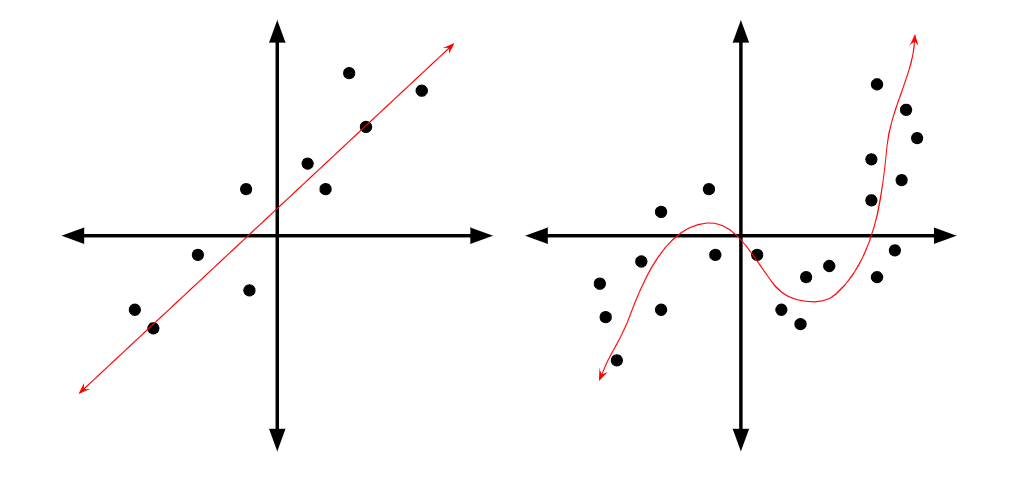
\includegraphics[scale=0.7]{../assets/line_best_fit.png}
\end{center}
The error, as mentioned, is defined by $r_i = y_i - p(t_i)$, where $y_i$ is the exact value and $p(t_i)$ is the value of the function (the estimate). Then, the $r_i$'s generate a vector known as the \textbf{residual} vector.

\subsection{Problem Statement}
Our goal is to find a $p(t) = a_0 + a_1 t$ such that $r \in \R^a$ is as small as possible. Hence, it turns into finding $a_0, a_1$ to minimize $||r||_2$. 

\subsubsection{Matrix Notation}
Let's begin by converting 
\[r_i = y_i - p(t_i) = y_i - (a_0 + a_1 t_i) = y_i - a_0 - a_1 t_i \quad i = 1, 2, \hdots, n\]
into matrix notation. This gives us 
\[\underbrace{\begin{bmatrix}
    r_1 \\ r_2 \\ \vdots \\ r_n
\end{bmatrix}}_{\rr \in \R^n} = \begin{bmatrix}
    y_1 - a_0 - a_1 t_1 \\ 
    y_2 - a_0 - a_1 t_2 \\ 
    \vdots \\ 
    y_n - a_0 - a_1 t_n
\end{bmatrix} = \begin{bmatrix}
    y_1 \\ y_2 \\ \vdots \\ y_n
\end{bmatrix} \begin{bmatrix}
    a_0 + a_1 t_1 \\ 
    a_0 + a_1 t_2 \\
    \vdots \\ 
    a_0 + a_1 t_n
\end{bmatrix} = \underbrace{\begin{bmatrix}
    y_1 \\ y_2 \\ \vdots \\ y_n
\end{bmatrix}}_{\y \in \R^n} - \underbrace{\begin{bmatrix}
    1 & t_1 \\ 
    1 & t_2 \\ 
    \vdots & \vdots \\ 
    1 & t_n
\end{bmatrix}}_{A \in \R^{n \times m}} \underbrace{\begin{bmatrix}
    a_0 \\ a_1
\end{bmatrix}}_{\x \in \R^{m}}\]
So, with the above matrix notation, also represented by 
\[\rr = \y - A\x,\]
the goal is to find an $\x \in \R^m$ such that $||\rr||_2$ is minimized. Essentially, 
\[\min_{x \in \R^m} ||\rr||_2 = \min_{x \in \R^m} ||\y - A\x||_2.\] Here, 
\begin{itemize}
    \item $n$ is the number of datapoints, and
    \item $m$ is the number of unknowns from the function. 
\end{itemize} 
\textbf{Remarks:}
\begin{itemize}
    \item $A$ is not squared.
    \item $n > m$.
\end{itemize} 
There will be no solutions\footnote{$A$ has more rows than columns.} to $A\x = \y$. Instead, we want to find $\x$ that minimizes the overall error.

\subsection{Other Basis Functions}
Instead of linear functions $p(t) = a_0 + a_1 t$, we an try other types of functions. For example, consider polynomials, or \[p(t) = a_0 + a_1 t + a_2 t^2 + \hdots + a_k t^k = \sum_{i = 0}^{k} a_i t^i.\] Here, $t^0 = 1$ and we have $(k + 1)$ unknowns. The matrix formulation is given by

\[\underbrace{\begin{bmatrix}
    r_1 \\ r_2 \\ \vdots \\ r_n
\end{bmatrix}}_{r \in \R^n} = \begin{bmatrix}
    y_1 - p(t_1) \\ 
    y_2 - p(t_2) \\ 
    \vdots \\ 
    y_n - p(t_n)
\end{bmatrix} = \begin{bmatrix}
    y_1 \\ y_2 \\ \vdots \\ y_n
\end{bmatrix} - \begin{bmatrix}
    p(t_1) \\ p(t_2) \\ \vdots \\ p(t_n)
\end{bmatrix} = \underbrace{\begin{bmatrix}
    y_1 \\ y_2 \\ \vdots \\ y_n
\end{bmatrix}}_{\y \in \R^n} - \underbrace{\begin{bmatrix}
    1 & t_1 & t_1^2 & \hdots & t_1^k \\ 
    1 & t_2 & t_2^2 & \hdots & t_2^k \\ 
    \vdots & \vdots & \vdots & \ddots & \vdots \\ 
    1 & t_n & t_n^2 & \hdots & t_n^k
\end{bmatrix}}_{A \in \R^{nn \times (k + 1)}} \underbrace{\begin{bmatrix}
    a_0 \\ a_1 \\ \vdots \\ a_k
\end{bmatrix}}_{\x \in \R^{k + 1}}.\]

Here, $\rr = \y - A\x$ is called the \emph{residual}. To solve this, we will use the QR decomposition. 

\subsection{QR Decomposition}
In essence, QR decomposition states that we can decompose a matrix $A$ into two matrices, $Q$ and $R$, such that 
\[A = QR,\]
where $Q$ is orthogonal and $R$ is upper-triangular. 

\subsubsection{A Brief Review}
\begin{definition}{Orthogonal Matrix}{}
    $Q \in \R^{n \times n}$ is called \textbf{orthogonal} if $Q^T = Q^{-1}$, i.e., $Q^T Q = QQ^T = I$. 
\end{definition}

\begin{mdframed}
    (Example.) Consider the rotations in $\R^n$. Note that 
    \[Q = \begin{bmatrix}
        \cos\theta & -\sin\theta \\ 
        \sin\theta & \cos\theta
    \end{bmatrix} \quad Q^T = \begin{bmatrix}
        \cos\theta & \sin\theta \\ 
        -\sin\theta & \cos\theta 
    \end{bmatrix}.\]
    It follows that \[QQ^T = \begin{bmatrix}
        1 & 0 \\ 0 & 1
    \end{bmatrix} = I.\]
\end{mdframed}

\begin{theorem}{}{}
    If $Q \in \R^{n \times n}$ is an orthogonal matrix, then 
    \begin{enumerate}
        \item $\cyclic{Q\x, Q\y} = \cyclic{\x, \y}$. 
        \item $||Q\x||_2 = ||\x||_2$.
    \end{enumerate}    
\end{theorem}
It might be useful to consider this visualization: 
\begin{center}
    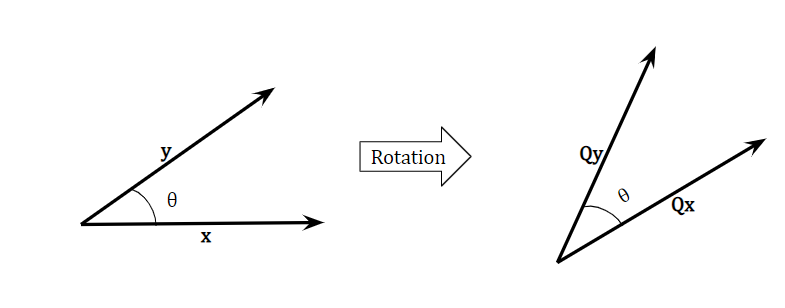
\includegraphics[scale=0.8]{../assets/angle_orth.png}
\end{center}

\begin{proof}
    We'll prove each part. 
    \begin{enumerate}
        \item $\cyclic{Q\x, Q\y} = (Q\x)^T Q\y = \x^T Q^T Q \y = \x^T \y = \cyclic{\x, \y}$. 
        \item $||Q\x||_2 = \sqrt{\cyclic{Q\x, Q\y}} = \sqrt{\cyclic{\x, \x}} = ||\x||_2$. 
    \end{enumerate}
    Thus, we're done.
\end{proof}

\subsubsection{QR Decomposition}
\begin{theorem}{}{}
    Let $A \in \R^{n \times m}$ such that $n \geq m$. Then, there exists an orthogonal $Q \in \R^{n \times m}$ and $R \in \R^{n \times m}$ with 
    \[R = \begin{bmatrix}
        r_{11} & r_{12} & \hdots & r_{1m} \\ 
        0 & r_{22} & \hdots & r_{2m} \\
        0 & 0 & \hdots & r_{3m} \\ 
        \vdots & \vdots & \ddots & \vdots \\ 
        0 & 0 & \hdots & r_{nm} \\ 
        0 & 0 & \hdots & 0 \\ 
        0 & 0 & \hdots & 0 \\ 
        0 & 0 & \hdots & 0 \\ 
        \vdots & \vdots & \ddots & 0 \\ 
        0 & 0 & \hdots & 0
    \end{bmatrix} = \begin{bmatrix}
        \hat{\R} \\ 0
    \end{bmatrix},\]
    with $\hat{\R} \in \R^{m \times m}$ being an upper-triangular matrix and the 0 being the zero-matrix.
\end{theorem}
Later on, we'll talk more about QR decomposition and solving the Least Squares Problem.

\end{document}